\documentclass[11pt,a4paper]{article}

\usepackage[margin=2.4cm]{geometry}
\usepackage{amsmath,amssymb}
\usepackage{booktabs}
\usepackage{graphicx}
\usepackage{listings}
\usepackage{xcolor}
\usepackage[hidelinks]{hyperref}
\usepackage{longtable}

\lstset{
  basicstyle=\ttfamily\scriptsize,
  breaklines=true,
  columns=fullflexible,
  frame=single,
  rulecolor=\color{gray!40},
  backgroundcolor=\color{gray!5},
  xleftmargin=6pt,
  framexleftmargin=6pt,
}

\newcommand{\task}[1]{\texttt{#1}}

\title{Five Tasks for Agents' Last Exam:\\
       Metrics, Calibration, and What Measurement Overturned}
\author{Pengcheng Xu \\ \texttt{px6@illinois.edu}}
\date{15 August 2026}

\begin{document}
\maketitle

\begin{abstract}
This note documents five candidate tasks contributed to Agents' Last Exam, the
scoring function used by each, and the calibration procedure that produced their
difficulty numbers. Its more useful content is negative. Four separate assumptions
about what makes a task hard were measured and found false, two shipped tasks
contained exploits that paid a substantial score for no work, and one task's
reported difficulty turned out to be manufactured by an ambiguity in the task rather
than by the problem. Every number here was produced by running a frontier agent
through each task's own \texttt{start()} hook and scoring with its own grader, and
each is reported with the check that established it was not an artefact.
\end{abstract}

\section{The tasks}

\begin{center}
\small
\begin{tabular}{@{}llrl@{}}
\toprule
Task & Domain & Measured & Reading \\
\midrule
\task{gen1\_battle\_engine\_reconstruction} & computing\_math & $0.000$ ($n{=}3$) & last-exam candidate \\
\task{minecraft\_excavation\_procedure}     & computing\_math & $0.471$          & discriminating \\
\task{kart\_telemetry\_extraction}          & visual\_media   & $0.116$          & hard; licence conflict \\
\task{eval\_harness\_leakage\_audit}        & computing\_math & $0.833$ ($n{=}3$) & near-term \\
\task{lockstep\_desync\_repro}              & computing\_math & $1.000$          & below near-term \\
\bottomrule
\end{tabular}
\end{center}

All five share a shape: the agent is given behaviour and must recover the rule that
produced it, then is graded on held-out instances of that rule. None ships a
normative specification, for reasons Section~\ref{sec:spec} makes precise.

\section{Scoring functions}

\subsection{Exact reproduction with per-family diagnosis (\task{gen1})}

A submission is an engine. It is run on each held-out scenario and its output
compared byte for byte against the reference engine's protocol log and final battle
state. Writing $F$ for the set of mechanic families and $S_f$ for the scenarios in
family $f$,
\begin{align}
\mathrm{exact}(s) &= \mathbb{1}\!\left[\text{log}(s) = \text{log}^{\star}(s)\ \wedge\ \text{state}(s) = \text{state}^{\star}(s)\right], \\
\mathrm{mechanics} &= \frac{1}{|F|}\sum_{f \in F} \prod_{s \in S_f} \mathrm{exact}(s),
\qquad
\mathrm{full\_pass} = \prod_{s} \mathrm{exact}(s).
\end{align}
There is no tolerance. \textsc{mechanics} is the reported score; it names which
families broke, which \textsc{full\_pass} alone cannot. Its known limitation is that
it only discriminates above a threshold: a wrong core damage formula fails every
family simultaneously, so the per-family diagnostic becomes informative only once
the core is right.

\subsection{Rank gate times absolute accuracy (\task{kart})}

Ranking races correctly is cheap and counting correctly is not, so rank agreement is
used only as a gate. For dimension $d$ over races $r$, with $\tau$ Kendall's
concordant-minus-discordant statistic and $\mathrm{tol}(g) = \max(1, 0.3\,|g|)$,
\begin{align}
\mathrm{acc}_d &= \frac{1}{|R|}\sum_{r \in R} \max\!\left(0,\ 1 - \frac{|p_{d,r} - g_{d,r}|}{\mathrm{tol}(g_{d,r})}\right), \\
\mathrm{score}_d &= \mathrm{clamp}(\tau_d, 0, 1)\cdot \mathrm{acc}_d,
\qquad
\mathrm{reward} = \frac{\sum_d w_d\,\mathrm{score}_d}{\sum_d w_d}.
\end{align}

A defect worth recording: $\tau$ was first normalised over \emph{all} race pairs.
Several races share a spin-out count, so ground-truth ties sat in the denominator
while contributing nothing to the numerator, and \textbf{the exact ground truth
scored below $1.0$ as a submission}. The positive control caught it. $\tau$ now
excludes pairs the truth cannot order:
\begin{equation}
\tau_d = \frac{\#\{(i,j) : \Delta g \cdot \Delta p > 0\} - \#\{(i,j) : \Delta g \cdot \Delta p < 0\}}
              {\#\{(i,j) : g_{d,i} \neq g_{d,j}\}}.
\end{equation}
A pair the truth orders but the prediction ties still earns nothing, so this is not
a loophole.

\subsection{Repair and proof, halved (\task{eval\_harness\_leakage\_audit})}

The agent must repair five leakage defects \emph{and} demonstrate the repairs with a
test suite. With $P$ the hidden behavioural probes and $M$ the defect mutants,
\begin{equation}
\mathrm{fixes} = \frac{1}{|P|}\sum_{p \in P} \mathbb{1}[p \text{ passes}],
\qquad
\mathrm{kills} = \mathbb{1}[\text{suite passes the reference}] \cdot \frac{1}{|M|}\sum_{m \in M} \mathbb{1}[\text{suite fails } m],
\end{equation}
\begin{equation}
\mathrm{reward} = \tfrac{1}{2}\,\mathrm{fixes} + \tfrac{1}{2}\,\mathrm{kills}.
\end{equation}
The gate on \textsc{kills} is the anti-gaming control: a suite of \texttt{assert
False} kills every mutant, so it must first pass a known-correct harness.

\subsection{Exact worlds plus overlap (\task{minecraft})}

For held-out worlds $W$, with $D(w)$ the set of cells a run cleared,
\begin{equation}
\mathrm{reward} = \frac{1}{2}\underbrace{\frac{1}{|W|}\sum_{w} \mathbb{1}\!\left[A_w = A^{\star}_w\right]}_{\text{exact}}
                + \frac{1}{2}\underbrace{\frac{1}{|W|}\sum_{w} \frac{|D(w) \cap D^{\star}(w)|}{|D(w) \cup D^{\star}(w)|}}_{\text{Jaccard}}.
\end{equation}
The partial term was chosen by measuring what each candidate pays a bot doing no
real work (Table~\ref{tab:mcmetric}). Per-cell accuracy is disqualified outright:
most of the arena is untouched by the procedure anyway, so idleness scores well.

\begin{table}[h]
\centering
\small
\caption{Choosing the partial-credit term by what it pays for nothing.}
\label{tab:mcmetric}
\begin{tabular}{@{}lrr@{}}
\toprule
Partial term & does nothing & digs everything \\
\midrule
per-cell accuracy   & ${\sim}0.5$ & low \\
F1 over dug cells   & $0.000$ & $0.264$ \\
\textbf{Jaccard over dug cells} & $\mathbf{0.000}$ & $\mathbf{0.183}$ \\
\bottomrule
\end{tabular}
\end{table}

\section{Calibration procedure}

Each task is staged through its own \texttt{start()} hook into a scratch directory,
an agent is run there exactly as the harness would run one on a VM, and the result
is scored by the task's own grader. The only thing absent relative to a real run is
the VM.

\begin{center}
\small
\begin{tabular}{@{}ll@{}}
\toprule
harness & Codex CLI 0.145.0, \texttt{codex exec}, sandbox \texttt{workspace-write} \\
model & \texttt{gpt-5.6-sol} \\
reasoning effort & \texttt{xhigh} \\
\bottomrule
\end{tabular}
\end{center}

This agent is \emph{stronger} than the reference point Agents' Last Exam classifies
against (Sonnet 4.6 or GPT-5.5 at low or medium effort). Failures here are therefore
conservative: if this agent cannot solve a task, a weaker one will not either. A
solve here, by contrast, is conclusive that a task is easy.

Two disciplines are applied to every number. An exact $0.000$ is the signature of a
broken interface, so it is not reported until the run is shown to have executed
cleanly; an exact $1.000$ gets the same treatment in reverse. And every shortcut a
task's structure makes available is measured, not argued about.

\section{What measurement overturned}

\subsection{Withholding a specification is an effort lever, not a difficulty lever}
\label{sec:spec}

\task{lockstep\_desync\_repro} was built on the premise that removing its
specification would make it hard. Measured:

\begin{center}
\small
\begin{tabular}{@{}llrr@{}}
\toprule
Condition & Mechanics & Elapsed & Score \\
\midrule
full specification & 5 planted deviations & 315\,s & $1.000$ \\
\textbf{no specification} & same & 2374\,s & $\mathbf{1.000}$ \\
no specification (\task{gen1}) & 48 move effects, rotated crit test & 5528\,s & $\mathbf{0.000}$ \\
\bottomrule
\end{tabular}
\end{center}

Deleting the specification cost $7.5\times$ in wall time and changed the score by
zero. Rows two and three hold ``no specification'' constant and vary only the size
of the mechanical surface, and the outcome flips completely. \textbf{Difficulty
comes from the mechanical surface, not from withholding documentation.}

\subsection{The same finding, paid for twice}

\task{minecraft\_excavation\_procedure} v1 used three marker types and one
conditional exception, and was solved at $1.000$ on the first attempt in 1100\,s.
The cause was structural: each marker's effect was independent and additive, so
every rule could be inferred alone from a single before/after pair. Marker density
had been tuned so the conditional appeared nine times in the examples; it made no
difference.

v2 changes exactly the two things the measurement above supports. Effects are
applied in a hidden order with each seeing the world the previous ones left, so no
rule can be read off in isolation; and the surface grows to eight marker types
including a suppressor, a parity gate and a fixpoint closure. Evidence was
\emph{widened} from 8 worked examples to 40, on the principle that difficulty should
come from the size of the hypothesis space rather than from starving the agent.
Measured: $0.471$, with 1 of 16 worlds exact and mean overlap $0.879$.

\subsection{A task can manufacture difficulty from its own ambiguity}

\task{eval\_harness\_leakage\_audit} first measured $0.500, 0.500, 1.000$. Reading
what the losing submissions actually asserted showed that one lost the proof half by
requiring the mathematical median of an even-sized column, where the reference used
the upper of the two middle values, a convention the task never stated. That is the
task penalising a disagreement it had failed to specify. Fixed at the root, three
fresh runs give $0.500, 1.000, 1.000$: the corrected task is \emph{easier} than the
one it replaced, which is the honest direction of the correction.

\subsection{Controls must come from the structure, not from a list}

\task{kart\_telemetry\_extraction} first paired its two halves by track: the same
twelve tracks appeared in both, raced twice. A track raced twice yields similar
telemetry, so

\begin{center}
\small
\begin{tabular}{@{}lr@{}}
\toprule
No-video submission, original split & reward \\
\midrule
copy the labelled value for the matching track & $\mathbf{0.257}$ \\
\bottomrule
\end{tabular}
\end{center}

with no video decoded at all. The agent that had actually built detectors scored
$0.337$, so its real margin was $0.080$, and on \texttt{skid\_time} the copy was
\emph{more accurate} ($0.715$) than the agent ($0.647$). The rank gate does not catch
this because track identity genuinely correlates with the counts. The split is now
track-disjoint and the best no-video submission scores $0.000$.

The controls in place at the time tested a constant answer and a rank-only answer.
Neither expresses ``copy the labelled half'', which is the obvious exploit the moment
two halves share a key. \textbf{A control has to be derived from the specific
structure a task hands the agent.}

\section{Prompt examples}

Task descriptions are the only statement of the rules that exists in three of the
five tasks. Two are reproduced in the form the agent receives them, abridged.

\subsection{\task{gen1\_battle\_engine\_reconstruction}}

\begin{lstlisting}
Reconstruct a battle engine from its observed behaviour.

Under `input/` is a corpus of battles from a deterministic Generation I battle
engine. You are given no specification: no damage formula, no critical-hit rule, no
random-number consumption order, no turn order. The corpus is the only statement of
the rules that exists.

- corpus/scenarios.json: 638 scenarios. Each carries the roll tape it used as hex,
  the exact starting battle state, the move each side selected, and an update cap.
- corpus/expected.json: the protocol log the engine emitted on every update, and the
  final battle state.
- docs/protocol.json: names every event the engine can emit. It does not say when
  any of them happen.
- docs/layout.json: field offsets and sizes. It does not say what changes any of them.

Your engine is invoked once per scenario as `python3 engine.py <scenario.json>`.

Comparison is exact, byte for byte, on both the protocol log and the final state.
There is no tolerance.
\end{lstlisting}

\subsection{\task{minecraft\_excavation\_procedure}}

\begin{lstlisting}
Work out what a bot did to a world, then write a bot that does the same thing.

Under `input/` is `examples.json`: several worlds recorded before and after a
reference bot acted on each one. You are told nothing about what the bot did. The
transformation is a fixed procedure, identical in every example, and it is the only
thing that separates `before` from `after`.

Each world is a 9x9 arena of blocks, one layer, addressed by offset from its centre
as "dx,dz" with dx and dz from -4 to 4.

Write `output/bot.js`, a CommonJS module exporting run(arena):

    module.exports = { run: async function (arena) { ... } }

Your bot connects without operator rights, so server commands are unavailable:
whatever the procedure does, your bot has to do it by acting in the world.

Half the score is the fraction of worlds reproduced exactly, cell for cell; the
other half is the overlap between the set of cells you changed and the set the
reference changed.
\end{lstlisting}

\section{Task pipelines}

\begin{figure}[h]
\centering
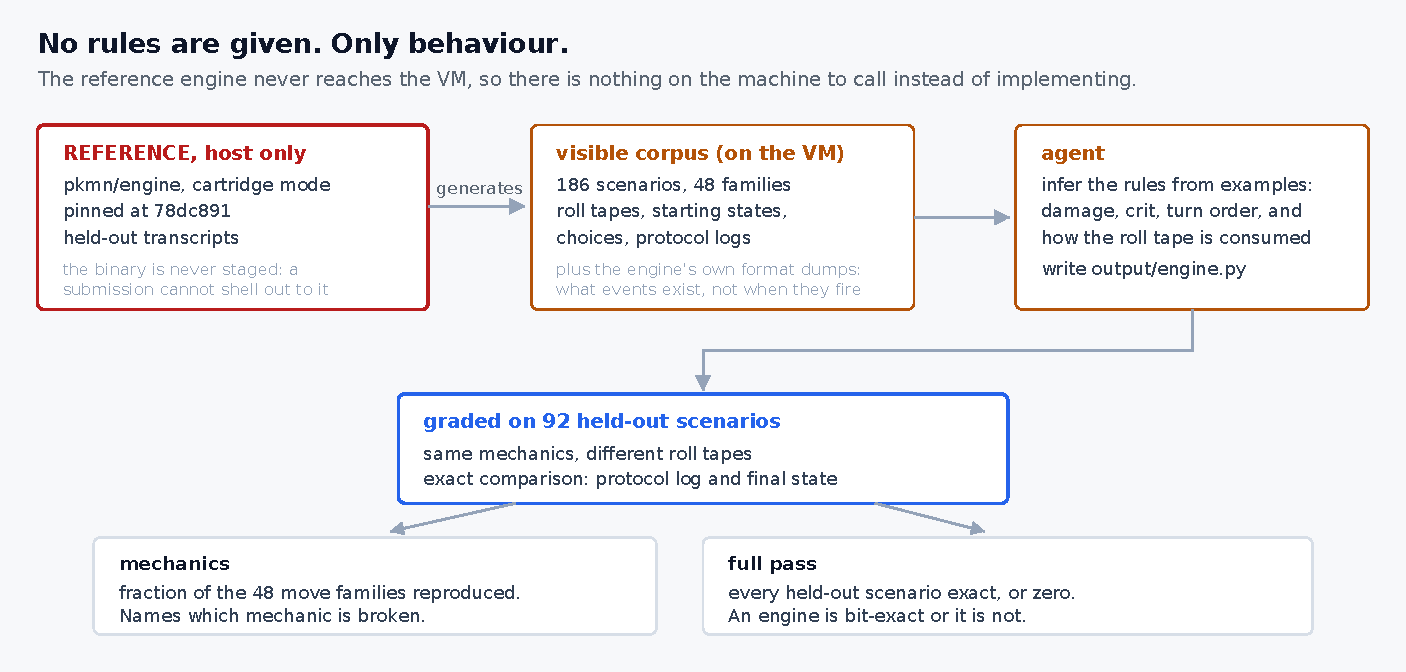
\includegraphics[width=\linewidth]{figures/gen1.pdf}
\caption{\task{gen1\_battle\_engine\_reconstruction}. The reference engine never
reaches the VM, so there is nothing on the machine to call instead of implementing
it.}
\end{figure}

\begin{figure}[h]
\centering
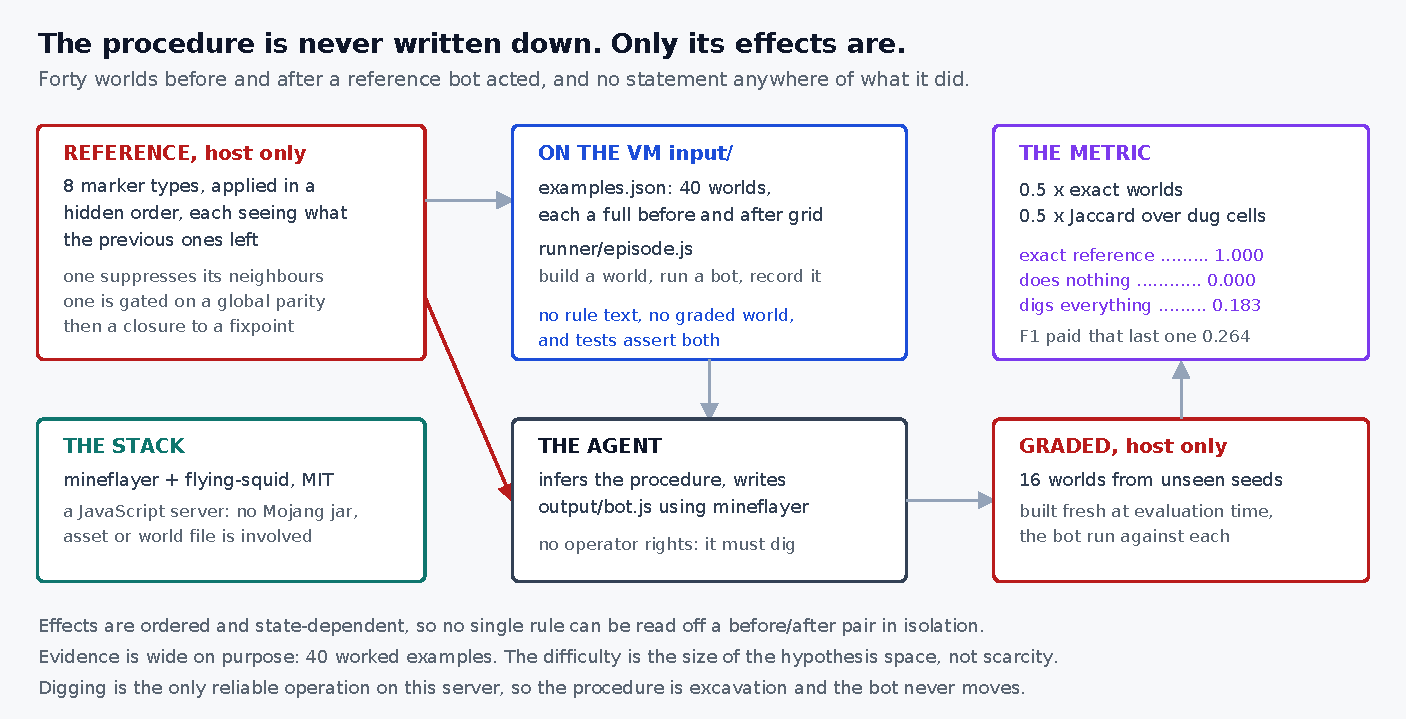
\includegraphics[width=\linewidth]{figures/minecraft.pdf}
\caption{\task{minecraft\_excavation\_procedure}. Effects are ordered and
state-dependent, so no single rule can be read off a before/after pair in isolation.}
\end{figure}

\begin{figure}[h]
\centering
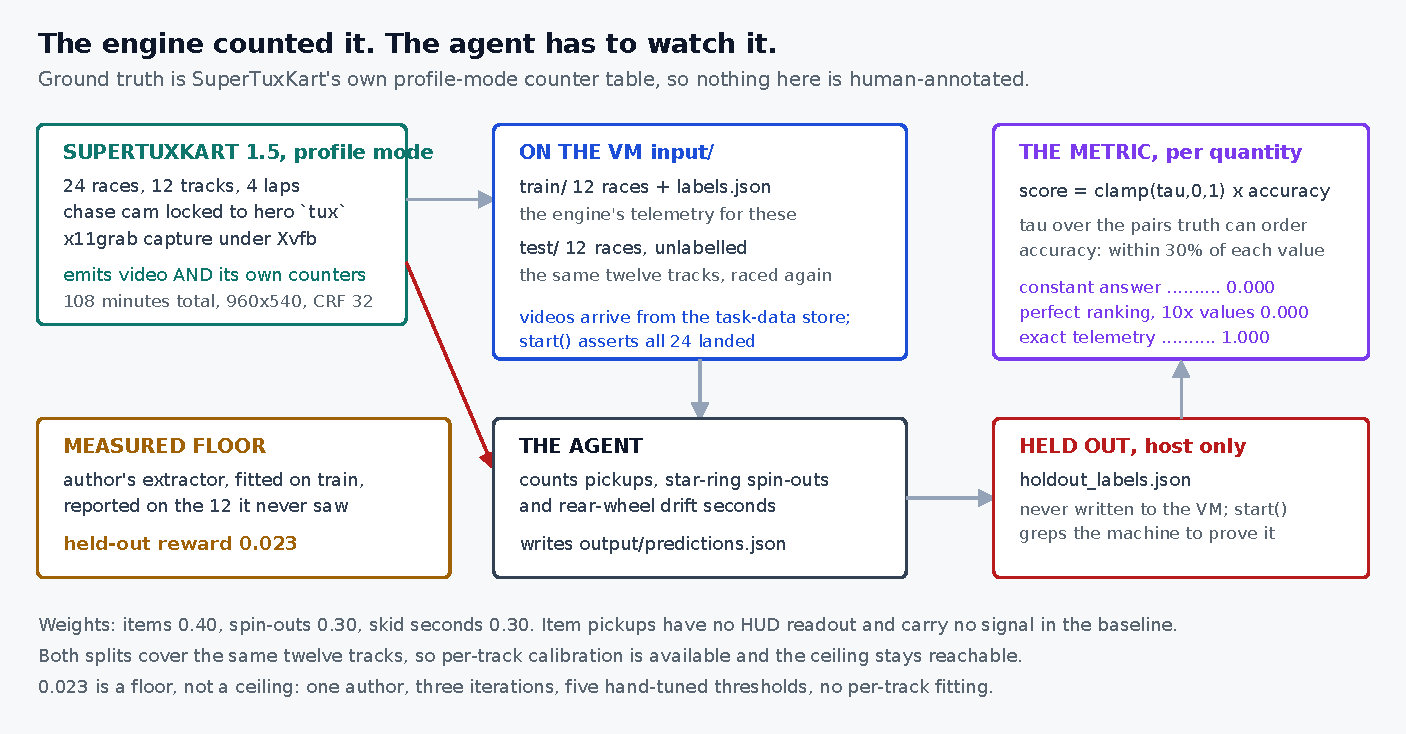
\includegraphics[width=\linewidth]{figures/kart.pdf}
\caption{\task{kart\_telemetry\_extraction}. Ground truth is the game engine's own
counter table, so nothing is human-annotated.}
\end{figure}

\begin{figure}[h]
\centering
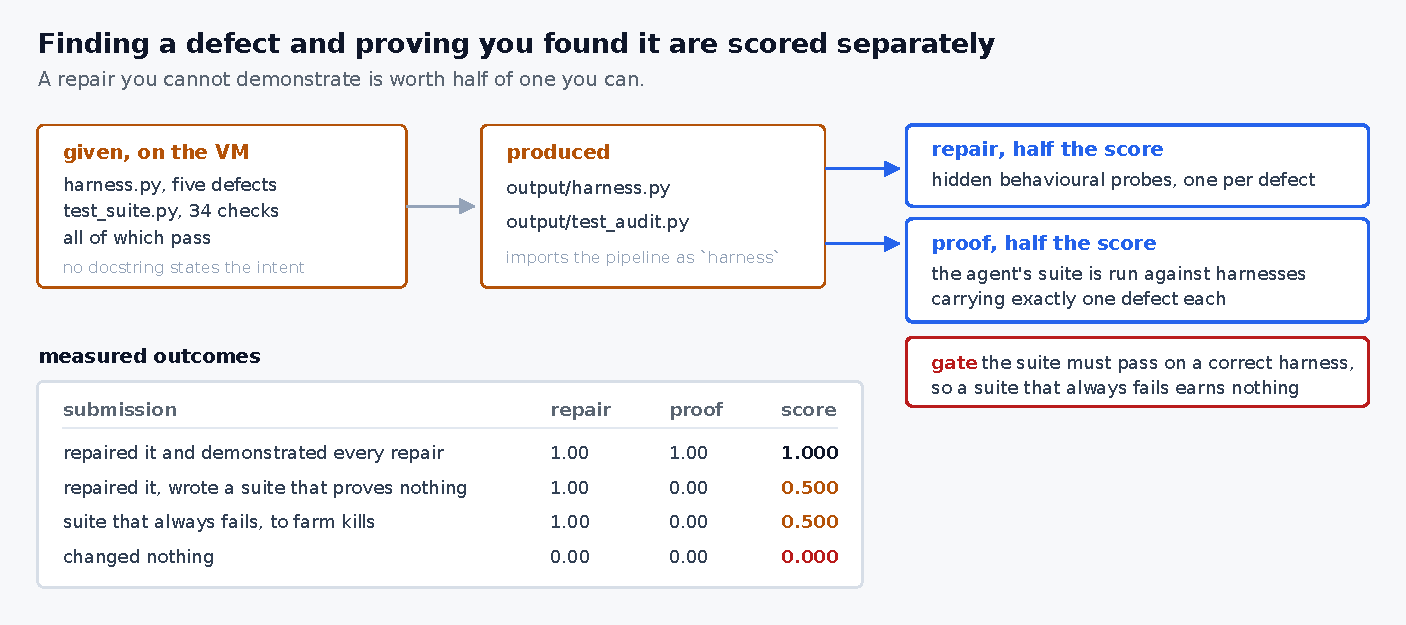
\includegraphics[width=\linewidth]{figures/audit.pdf}
\caption{\task{eval\_harness\_leakage\_audit}. Repairs are judged by hidden
behavioural probes; the test suite the agent writes is judged by what it detects.}
\end{figure}

\section{Licensing}

Task data must be licensable under CC BY 4.0. This is what decided the environment
for two of the five tasks and disqualified a third direction entirely.

\begin{center}
\small
\begin{tabular}{@{}lll@{}}
\toprule
Source & Licence & Consequence \\
\midrule
\texttt{pkmn/engine} & MIT & corpus is shippable \\
mineflayer, flying-squid, minecraft-data & MIT & environment is shippable \\
SuperTuxKart artwork & CC BY-SA & \emph{conflicts} with CC BY 4.0 \\
Minecraft gameplay video & proprietary & cannot be sublicensed at all \\
\bottomrule
\end{tabular}
\end{center}

The Minecraft task therefore uses \texttt{flying-squid}, an independent JavaScript
implementation of the protocol: no Mojang jar, asset, world file or account is
involved, and the only ``content'' is block type names, which are protocol
identifiers. A task built on recorded gameplay video could not carry the licence,
whatever its quality.

\section{Limitations}

\begin{itemize}
\item \textbf{\task{gen1} solvability is not fully proven.} Its positive control is a
Python shim that shells out to the reference engine, whereas the deliverable is a
self-contained Python file. Working from the shipped documents alone, the damage
pipeline was recovered and reproduces $28/28$ visible and $12/12$ held-out first-hit
damages exactly for two families, which shows the target is computable in the
required form. It does not show a full engine reaching $1.000$, and the bit
rotations involved were read from the reference source rather than derived from the
corpus.
\item \textbf{A text-only harness cannot calibrate a perception task.}
\texttt{codex exec} writes \texttt{ffmpeg} and NumPy but never sees a frame, so the
\task{kart} number measures the programmatic path only.
\item \textbf{Sample sizes are small.} $n{=}3$ for two tasks, $n{=}1$ for the rest.
None of these is a pass rate.
\item \textbf{A floor of zero cannot separate hard from unreasonable.} This is the
open question for \task{gen1} and the reason the limitation above matters.
\end{itemize}

\end{document}
